% Usenix submission:
%   13-pages, excluding bibliography and well-marked appendices
%   (no more than 16 pp. long)


\documentclass[letterpaper,twocolumn,10pt]{article}
\usepackage{usenix}
\usepackage[T1]{fontenc}
\usepackage[%
    breaklinks=true,colorlinks=true,linkcolor=black,%
     citecolor=black,urlcolor=black,bookmarks=true,bookmarksopen=false,%
    pdfauthor={},
    pdftitle={DDosCoin}
    ,pdftex]{hyperref}

\usepackage{amsmath,amssymb,amsbsy}
\usepackage{wasysym}
\usepackage{longtable}
\usepackage{mathptmx}\renewcommand{\ttdefault}{cmtt}
\usepackage[margin=0pt]{caption}
\usepackage{graphicx}
\usepackage{tikz}
\usepackage{xcolor}
\usepackage{tablefootnote}
\usepackage{longtable}
\usepackage{color}
\usepackage{url}\urlstyle{rm}
\usepackage[margin=1in]{geometry}
\usepackage{watermark}
\usepackage{booktabs}
\usepackage{listings}
\usepackage{cite}
\usepackage{paralist}
\usepackage{balance}
\usepackage{tabularx}
\usepackage[protrusion=true,expansion=true,kerning]{microtype}
\usepackage{algorithm, algorithmic}
\usepackage{multirow}
\usepackage{placeins}
\usepackage{pgfplots}
%\usepackage{wrapfig}
\usepackage{colortbl}
\usepackage{bigstrut}
\usepackage{subcaption}
\newcommand{\specialcell}[2][c]{%
  \begin{tabular}[#1]{@{}c@{}}#2\end{tabular}}
\usepackage{float}

\newcommand{\ind}{\hspace*{1em}}

%\hyphenpenalty=62

\marginparwidth 36pt
\newcommand{\mn}[1]{\marginpar{\scriptsize \raggedright #1}}

% Paragraph and subpar
\renewcommand{\paragraph}[1]{\medskip\noindent\textbf{#1}\quad}
\newcommand{\subpar}[1]{\medskip\noindent\textsl{#1}\enspace}

% Fix ugly USENIX subsection headings (AH 3/08)
\makeatletter
\renewcommand{\section}{\@startsection {section}{1}{\z@}%
                                   {-3.5ex plus-1ex minus -.2ex}%
                                   {2.3ex plus.2ex}%
                                   {\normalfont\large\bfseries}}
\renewcommand{\subsection}{\@startsection{subsection}{2}{\z@}%
                                     {-2.5ex plus-.7ex minus -.2ex}%
                                     {1.5ex plus .2ex}%
                                     {\normalfont\fontsize{11}{12.5}\bfseries}}
\makeatother

\clubpenalty10000

% Stop URLs from hyphenating after  "http:" (AH 12/08)
\def\UrlBreaks{\do-\do\.\do\@\do\\\do\!\do\_\do\|\do\;\do\>\do\]%
 \do\)\do\,\do\?\do\'\do+\do\=\do\#}
\def\UrlBigBreaks{\do\:\do\/}%

% TODO, TK, etc. (AH 4/12)
\usepackage{xspace}
\newcommand{\todo}[1]{{\color{red}{\textbf{\em [TODO: #1]}}}\xspace}
\newcommand{\TODO}[1]{\todo{#1}}
\newcommand{\tk}{{\color{red}{\bf TK}}\xspace}
\newcommand{\TK}{\tk}
\newcommand{\comment}[1]{\relax} % comment out text
\newcommand{\xcite}[1]{\relax} % comment out citation

    %\thiswatermark{\parbox{\textwidth}{\vskip30pt\centering
    %\vspace*{-20pt}%
    % This paper appeared in \emph{Proceedings of the 9th {\small USENIX} Workshop on Offensive Technologies (WOOT)}, August~2015.\\
    % Source code and an online demonstration are available at \href{https://keysforge.com/}{{\bf https://keysforge.com/}}.\\
    %\vskip6pt
    %\rule[\baselineskip]{\textwidth}{0.5pt}
    %}}


% Poor UTF support in LaTeX, stolen from http://tex.stackexchange.com/questions/279100/typeset-the-shrug-%C2%AF-%E3%83%84-%C2%AF-emoji
\newcommand{\shrug}[1][]{%
\begin{tikzpicture}[baseline,x=0.8\ht\strutbox,y=0.8\ht\strutbox,line width=0.125ex,#1]
\def\arm{(-2.5,0.95) to (-2,0.95) (-1.9,1) to (-1.5,0) (-1.35,0) to (-0.8,0)};
\draw \arm;
\draw[xscale=-1] \arm;
\def\headpart{(0.6,0) arc[start angle=-40, end angle=40,x radius=0.6,y radius=0.8]};
\draw \headpart;
\draw[xscale=-1] \headpart;
\def\eye{(-0.075,0.15) .. controls (0.02,0) .. (0.075,-0.15)};
\draw[shift={(-0.3,0.8)}] \eye;
\draw[shift={(0,0.85)}] \eye;
% draw mouth
\draw (-0.1,0.2) to [out=15,in=-100] (0.4,0.95); 
\end{tikzpicture}}


\pagestyle{plain}
\thispagestyle{empty}
\begin{document}

\title{DDoSCoin: Cryptocurrency with a Malicious Proof-of-Work}

\author{\rm{Eric Wustrow}\\
University of Colorado, Boulder\\
{\small ewust@colorado.edu}
}

\maketitle




\newcommand{\FigTx}{
\begin{figure*}[ht]
    \centering
    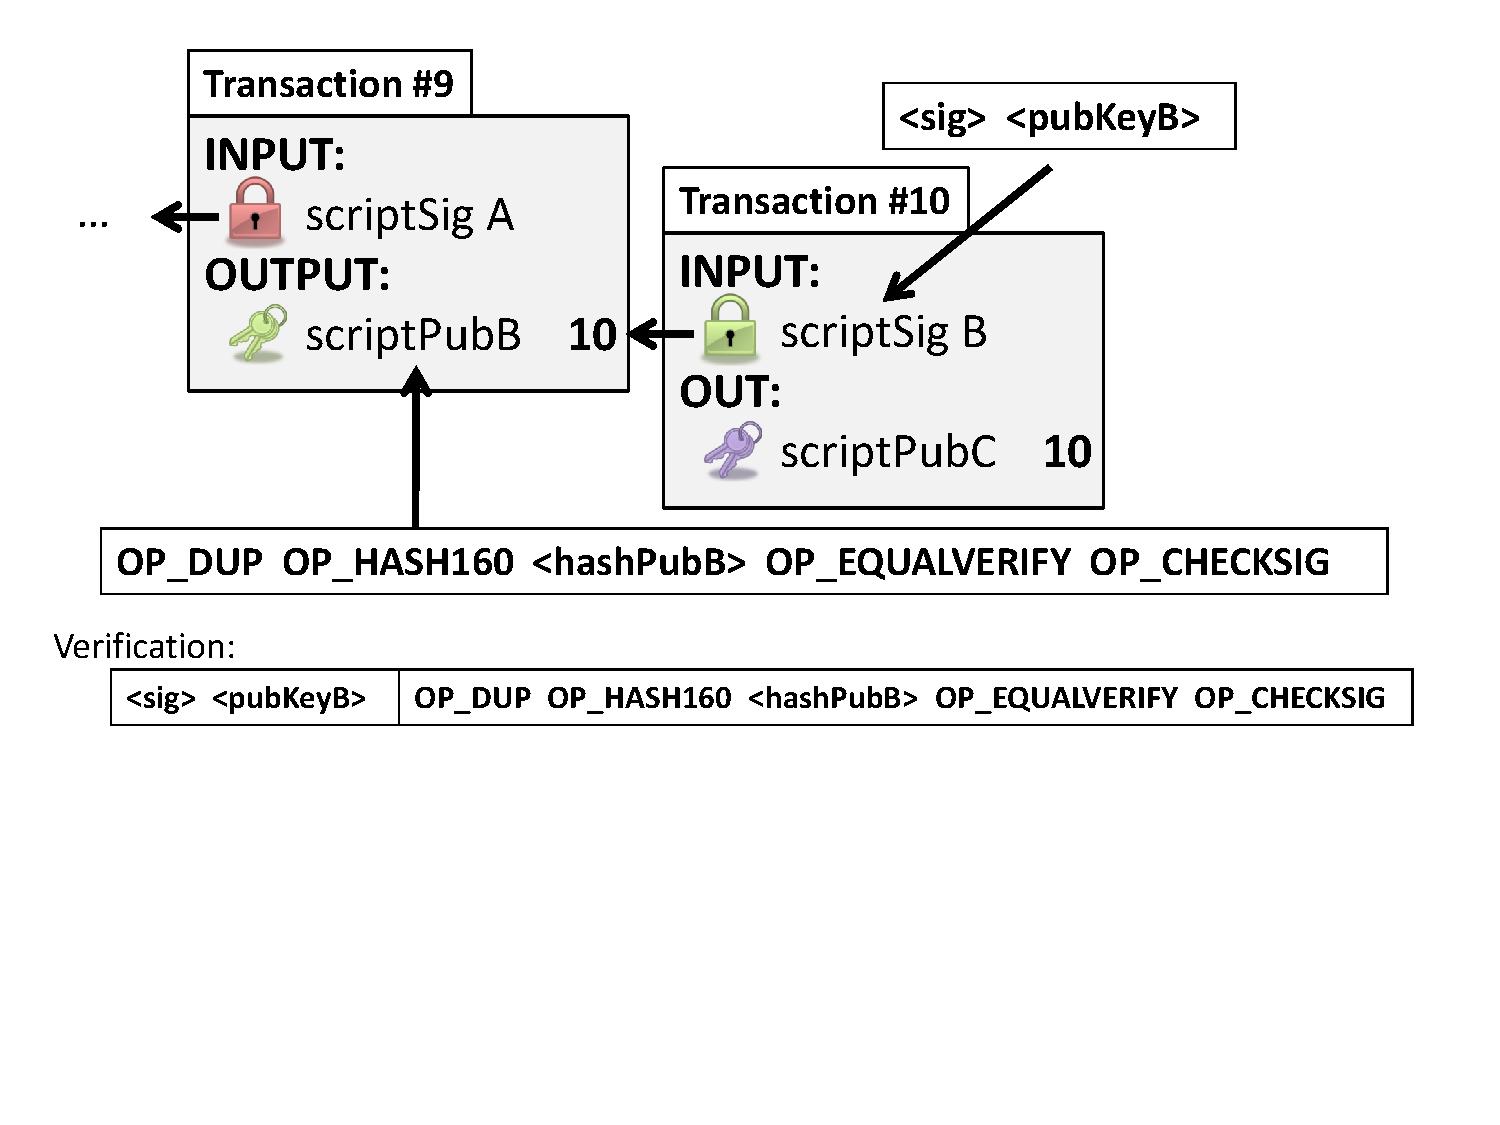
\includegraphics[width=0.9\textwidth,trim={0 6.5cm 1cm 0},clip]{btc-transaction.pdf}
    \caption{\textbf{Standard Bitcoin transaction script}\,--\, %
            Transaction \#10 spends \#9 by providing a
            valid input script that when prepended to Transaction \#9's output script,
            executes to produce a valid output. The output script stores a hash of a
            public key (verified using the OP\_DUP OP\_HASH160 and OP\_EQUALVERIFY opcodes),
            and requires a valid signature over the spending transaction (verified via
            OP\_CHECKSIG).}
    \label{fig:bitcoin-tx}
\end{figure*}
}

\newcommand{\FigTLS}{
\begin{figure*}[ht]
    \centering
    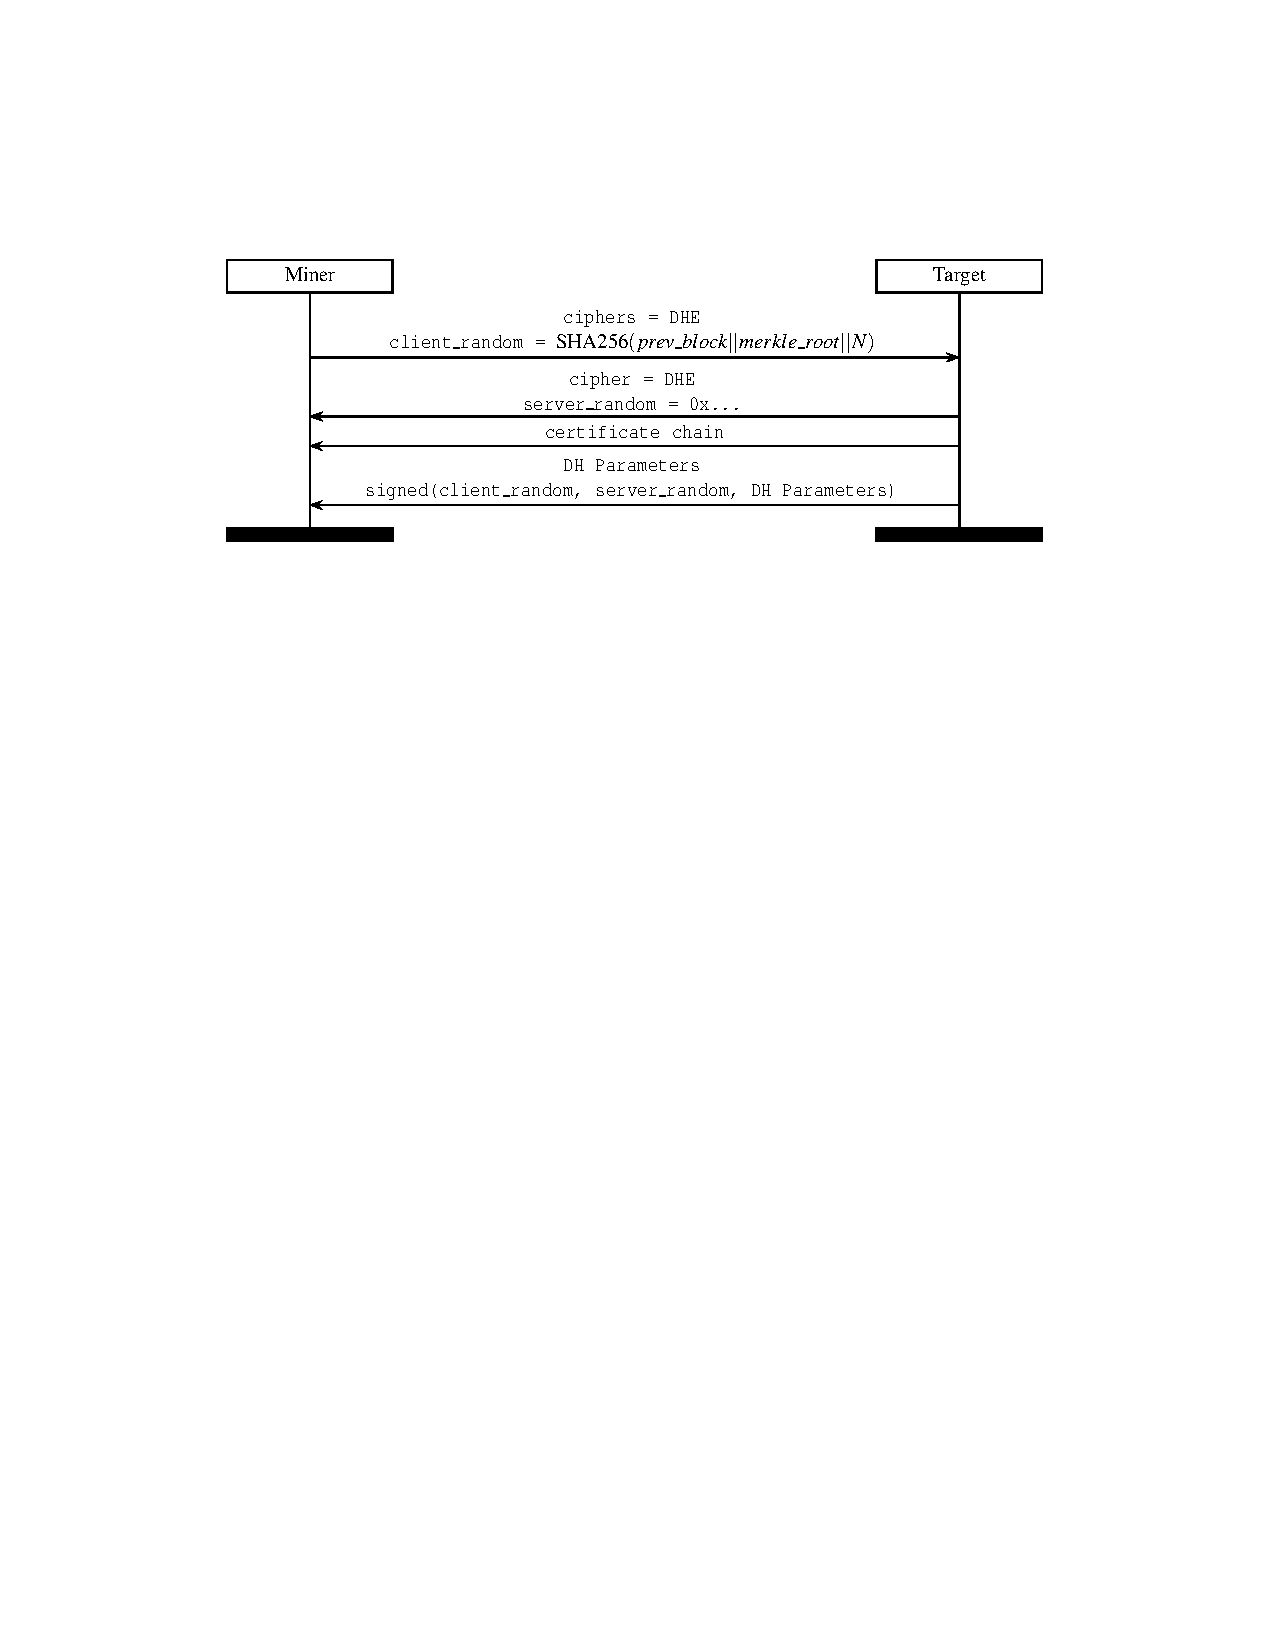
\includegraphics[width=0.9\textwidth,clip]{figures/tls.pdf}
    \caption{\textbf{Miner--Target Interaction}\,--\, %
	A single round-trip is required for each attempt to solve the proof-of-work. The client
	computes the \texttt{client\_random} to commit to a given previous block and set of 
	transactions, and only provides the server the option to use Diffie-Hellman Ephemeral
	cipher-suites. The server then calculates a signature dependent on the 
	\texttt{client\_random} and verifiable by the certificate the server provides.
}
    \label{fig:tls-connection}
\end{figure*}
}

\newcommand{\FigOverview}{
\begin{figure*}[ht]
    \centering
    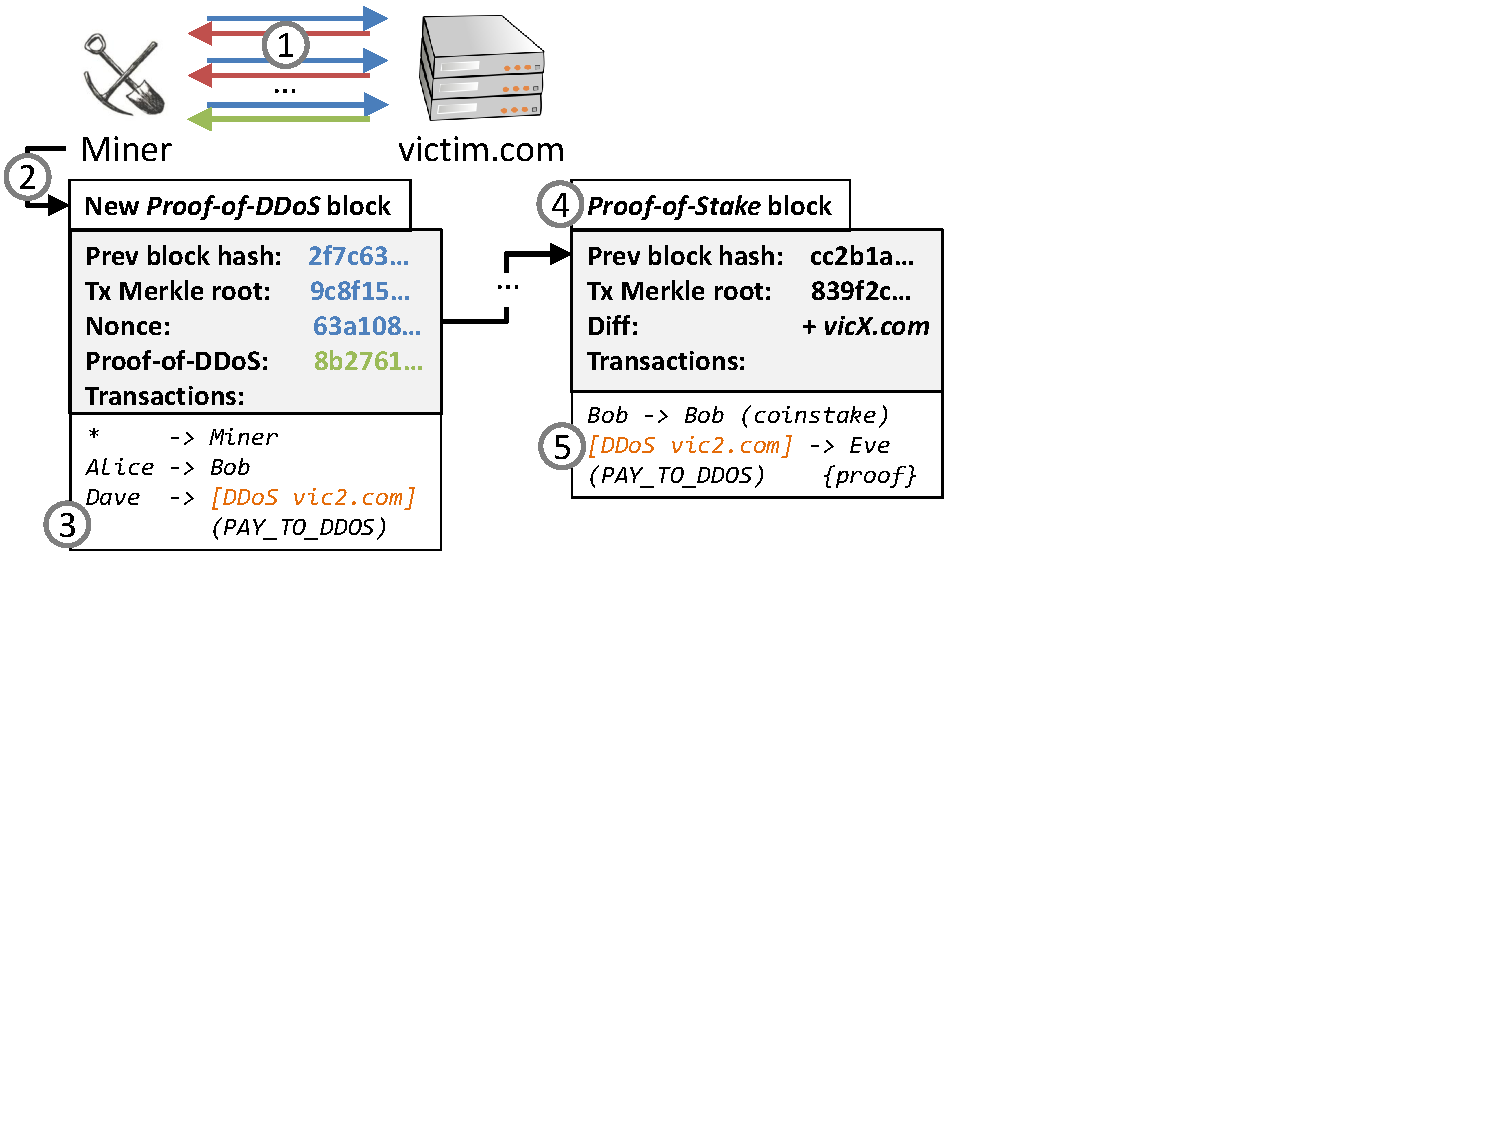
\includegraphics[width=0.9\textwidth,trim={0 9.5cm 9.2cm 0},clip]{ddoscoin-overview.pdf}
    \caption{\textbf{DDoSCoin Design}\,--\, %
    DDoSCoin miners make repeated connections to a victim server running TLSv1.2
\numcircledmod{1}. In each handshake, the miner commits to the previous block, a transaction
merkle root, and a secret nonce. Eventually the victim server will respond with
a signed message that meets the current proof-of-DDoS target difficulty, and the miner can
create a new block \numcircledmod{2} that includes this proof. Victim targets can be selected
in two ways: First, participants can pay into one-time bounties for specific
victims \numcircledmod{3}, which can be redeemed by anyone in a special PAY\_TO\_DDOS
transaction \numcircledmod{5} if they can provide a similar proof-of-DDoS against that victim. Second, the list of
valid victims that blocks can be mined for can be updated by proof-of-stake
blocks \numcircledmod{4}.}
    \label{fig:ddoscoin-overview}
\end{figure*}
}

\newcommand{\FigEval}{
\begin{figure}[t]
    \centering
    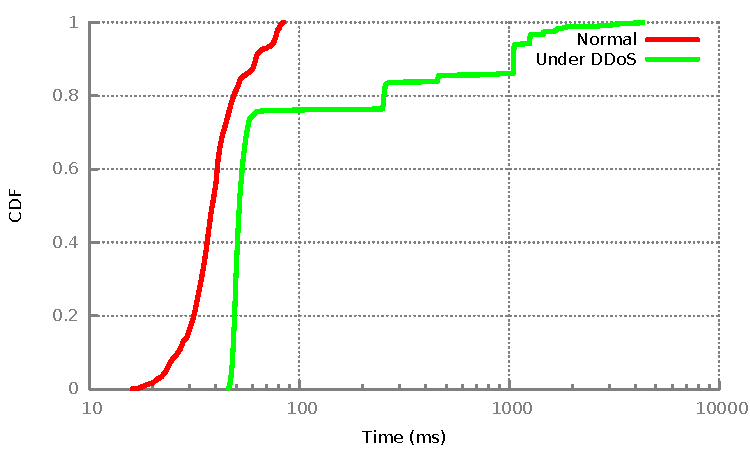
\includegraphics[width=0.9\linewidth]{../data/times.pdf}
    \caption{\textbf{DDoSCoin effect}\,--\, %
    We set up a quad-core nginx HTTPS server on a local network, and used Apache
benchmark (ab) to measure page load times under normal conditions (no DDoSCoin
miner running) and with a single DDoSCoin instance. DDoSCoin increases the
average page-load time 6-fold from 43ms to over 291ms.}
    \label{fig:eval}
\end{figure}
}



\begin{abstract}

Since its creation in 2009, Bitcoin has used a hash-based proof-of-work to
generate new blocks, and create a single public ledger of transactions. The
hash-based computational puzzle employed by Bitcoin is instrumental to its
security, preventing Sybil attacks and making double-spending attacks more
difficult. However, there have been concerns over the efficiency of this
proof-of-work puzzle, and alternative ``useful'' proofs have been proposed.

In this paper, we present DDoSCoin, which is a cryptocurrency with a
\emph{malicious} proof-of-work. DDoSCoin allows miners to prove that they have
contributed to a distributed denial of service attack against specific target
servers.  This proof involves making a large number of TLS connections to a
target server, and using infrequent cryptographic responses to prove that a
large number of connections has been made. Like proof-of-work puzzles, these
proofs are inexpensive to verify, and can be made arbitrarily difficult to
solve.

\end{abstract}




\section{Introduction}


Cryptocurrencies rely on proofs-of-work (PoW) that require miners to spend a
large amount of effort to solve a specific puzzle.  Solutions to these puzzles,
on the other hand, are designed to be inexpensive to verify. In Bitcoin, the
proof-of-work is a computational puzzle based on the SHA256 hash function, and
miners are tasked with finding a partial preimage. The best way to do this is to
iterate over a large number of inputs to the hash function, and check if the
output hash satisfies the partial preimage target. In simplified terms, to find
an input that hashes to N bits of 0s, the miner must perform on average $2^{N}$
hashes. Once such an input is found, other miners and Bitcoin nodes can verify the
puzzle solution with a single hash~\footnote{Bitcoin uses double-SHA256 in its
design, but this detail is not important for the purposes of this paper.}.


Although the proof-of-work used in Bitcoin gives it resistance to sybil attacks,
the amount of computational effort carried out collectively by its miners does
not contribute to any useful problems besides securing the currency from attack.
Indeed, this computational effort is substantial: As of 2016, miners
collectively perform roughly $10^{18}$ (or about $2^{60}$) hashes every
second~\cite{blockchain-hashrate}.

Many see this distributed computation as a colossal waste of CPU resources, and
researchers have proposed alternative cryptocurrencies (altcoins) that aim to
have more beneficial proofs-of-work~\cite{primecoin,permacoin} that provide
utility beyond securing the underlying currency, such as finding chains of
large primes or proving the archive of data. In this paper however, we
investigate going in the opposite direction, and propose an altcoin that has a
\emph{malicious} proof-of-work that is externally detrimental.

In particular, we propose a proof-of-work that allows miners to prove they have
participated in a distributed denial of service (DDoS) attack against a
particular target. Miners are incentivized to send and receive large amounts of network
traffic at the target in order to produce a valid proof-of-work. As in other
cryptocurrencies, these proofs can be inexpensively verified by others, and the
original miner can collect a reward. This reward can be sold for other
currencies (including Bitcoin or even traditional currencies), allowing botnet
owners and other attacks to directly collect revenue for their assistance
in a decentralized DDoS attack.


The malicious ``proof-of-DDoS'' operates by having miners create a large number of
TLS connections to a target webserver, and using the server's signed responses
as a proof of connection. In modern versions of TLS, the server signs a
client-provided parameter of the connection, along with server-provided values
used in the key exchange of the connection. This allows the client to prove to
others that it has communicated with the server. In addition, the signed value
returned by the server is not predictable to the client, and is randomly
distributed. Thus, clients can use a similar trick as in Bitcoin, and only
report connections that match some rare threshold, such as the signature from
the server starts with $N$ bits of 0s. On average, it will take clients $2^{N}$
connections to produce such a proof.

Although the malicious proof-of-DDoS only works against websites that support
TLS 1.2, as of April 2016, over 56\% of the Alexa top million websites support
this version of TLS~\cite{censys}. Furthermore, we
expect this number to increase as TLS support becomes more
widespread~\cite{letsencrypt}.

Using our proof-of-DDoS, we conceptualize a cryptocurrency that uses it, which
we call \emph{DDoSCoin}. In addition to using proof-of-DDoS, DDoSCoin allows
miners to select the victim servers by consensus using a proof-of-stake
protocol. Rather than specify a single website or static list that DDoSCoin
miners target, choosing them by consensus allows the choice of who is attacked
to be made collectively and fairly by DDoSCoin participants.

\emph{Contributions}
\begin{itemize}
\item Propose a novel conceptual cryptocurrency, DDoSCoin, whose proof-of-work
incentives miners to participate in a DDoS attack, and allows them prove they have done so.
\item Describe a way for target victims to be chosen by consensus of its
participants.
\item Implement our proof-of-work function and evaluate its performance and
impact.
\item Discuss several defenses against such a cryptocurrency that potential
victims can employ.
\end{itemize}

%Section blah does blah, and Section blat describes blat.

\section{Related Work}

Many alternate cryptocurrency protocols (altcoins) have been proposed since the
creation of Bitcoin. Although none have yet eclipsed the popularity of Bitcoin,
many altcoins have interesting innovations, often in the form of alternate
proof-of-work. For example, Litecoin uses scrypt in place of SHA256 in its
proof-of-work, with the intention of being ``ASIC-resistant'' in order to allow
anyone to mine competitively with only a CPU~\cite{litecoin}.

Permacoin is a proposed altcoin that uses a novel
\emph{proof-of-storage}~\cite{permacoin}.  Rather than waste computational
resources solving a useless proof-of-work puzzle (as in Bitcoin), miners are
instead incentivized to store parts of a large agreed-upon file. In order to be
competitive in Permacoin, miners prove that they can retreive an assigned
portion of the file.

In Primecoin, miners search for special chains of prime
numbers~\cite{primecoin}. Although Primecoin has found several large Cunningham
and bi-twin chains, it remains unclear if such primes have any practical use.

TorPath proposes a proof-of-bandwidth altcoin that incentivizes users to
participate in the Tor Network~\cite{torpath}. However, it relies on a set of
semi-trusted centralized servers to assign Tor circuits to clients. It is also
susceptible to collusion and sybil attacks by participants, however many of
these attacks are outside the threat model of TorPath as it requires performing
those attacks against the underlying Tor network. In contrast, DDoSCoin does not
require any centralized parties for the proof-of-DDoS, besides trusting existing
certificate authorities to validate domains.

Although Bitcoin uses a scripting language for transactions (see
Section~\ref{sec:scripting}), the allowed operations are very
limited~\cite{bitcoin-paper}. Ethereum allows transactions to be
\emph{programmable contracts}, whereby a programmer can specify in a custom
scripting language arbitrary logic, including conditional payments or
fee-collection. While the Ethereum Virtual Machine (EVM) that executes these
contracts does not provide external network access to the scripts, it could
still be used to implement some parts of DDoSCoin. For example, it is possible
to create an Ethereum contract that pays a bounty to anyone that can provide a
proof-of-DDoS for a specified target. This would effectively accomplish the same
outcome as PAY\_TO\_DDOS (described in Section~\ref{sec:pay-to-ddos}), and
implementing DDoSCoin's proof-of-DDoS verification.

%Other interesting proofs-of-work?  Botnet-as-a-service?

\section{Background}

In this section, we review relevant basics of cryptocurrency. For more
detail, we refer the reader to other
sources~\cite{bitcoin-book,bitcoin-paper,bitcoin-sok}.

\subsection{Cryptocurrency}
\label{sec:scripting}
\FigTx

Bitcoin employs a hash-based proof-of-work protocol to construct a public ledger
of transactions. In this protocol, miners attempt to solve a simple hash-based
computational puzzle in order to mine blocks. Mining a block nets the miner a
reward, and the right to specify what new (valid) transactions should be
included in the public ledger. To mine a block, a miner must find a hash of a
block header that is less than an adjustable target. The block header includes
the hash of the last block found, the Merkle root of the list of transactions
the miner wants to include in this block, and a nonce. The easiest way to solve
this puzzle is to iterate the nonce\footnote{or modify transactions, therby
changing the Merkle root} until the hash satisfies the target difficulty. Then,
the miner publishes the found block, and miners use this block as the latest
block.

Each block commits to a set of transactions, which each must be valid for the
block to be considered valid. Transactions in Bitcoin are scripts, and each new
transactions specifies an \emph{output script} that must be satisfied in order
for the coins
to be spent. For example, an output script might specify that it requires a
spending transaction to provide a valid signature, with the output script
specifying the public key to validate it with. To spend such a transaction
requires creating a new transaction that references the previous one, and
provides an input (scriptSig) that ``solves'' the previous transactions' output
(scriptPubKey); in this case, a valid signature over the new transaction. This
new transaction can then specify a new output (scriptPubKey) for these coins.
Figure~\ref{fig:bitcoin-tx} shows an example of a standard Bitcoin transaction
script.


\subsection{Proof-of-Stake}

Proof-of-Stake is an alternate way of generating new blocks in a cryptocurrency.
In this system, blocks are ``minted'' (rather than mined) based on how much
stake the miner has in the currency (rather than their fraction of computational
power). Proof-of-stake assumes that the underlying cryptocurrency is already
somewhat distributed, for example through prior use of a traditional
proof-of-work system. There are several variants on proof-of-stake; in this
subsection, we will describe Peercoin, an active alternate cryptocurrency that
employs a hybrid proof-of-work and proof-of-stake algorithm to mint blocks. For
more details on proof-of-stake, we refer the reader to the
Peercoin~\cite{peercoin} and NXT~\cite{nxt} whitepapers.

Peercoin's proof-of-stake allows currency holders to mint new blocks based on
how many coin-days they are able and willing to consume. ``Coin-days consumed''
is a measure of the product of the amount of coins spent in a transaction, and
the number of days since they were last spent. For example, to consume 10
coin-days, a currency holder can spend 10 Peercoin that they have held for a
day, or equivalently, spend 5 Peercoins that were last spent 2 days ago. Note
that the holder can send these coins to anyone (including themselves) in order
to consume the coin age.

To mint a new block, a minter creates a special transaction (presumably one
where the minter pays themself) where one of the inputs has been unspent for at
least 30 days. The resulting transaction, along with a timestamp, must meet a
certain hash target that gets easier proportional to how many coin-days are
consumed by the transaction. For example, if the current difficulty gives a
minter consuming 100 coin-days a 1\% chance of minting a block per second, a
minter that was able to consume 200 coin-days would have a 2\% chance per
second.

The input to the hash includes information about the ``aged'' transaction, as
well as a current timestamp\footnote{In recent versions of Peercoin, the hash
also includes a stakeModifier which is computed from recent blocks; however,
these details are not important for our purposes}. If this hash is less than the
current target multiplied by the number of coin-days consumed in the
transaction, then the transaction meets the proof-of-stake difficulty and a new
block is minted. Although this looks similar to a proof-of-work check where a
hash is being compared to a target, here the only varying inputs are the
long-lived (aged) input transaction, and a course-grained timestamp with a
resolution of 1 second. Thus, for each aged unspent transaction output they
control, minters perform only one hash per second in order to solve the
proof-of-stake.

% hash(nStakeModifier + txPrev.block.nTime + txPrev.offset + txPrev.nTime +
%       txPrev.vout.n + nTime) < bnTarget * nCoinDayWeight
%
% ss << nTimeBlockFrom << nTxPrevOffset << txPrev.nTime << prevout.n <<
%   nTimeTx;
% given a new tx that is going to be my "proof-of-stake" tx,
% which has an input from prevTx (where prevTx is at least 30 days old)
% H(nStakeModifier + txPrev.block.nTime + txPrev.offset + txPrev.nTime +
%   txPrev.vout.n + tx.nTime)

% stakeModifiers (in v0.3): you start from the block where txPrev was in,
% and then walk forward until the first block that was made more than
% GetStakeModifierSelectionInterval() seconds after that the block txPrev was in (about 8.8 days...)
% If that block has the stakeModifier flag set, use its stakeModifier


% Ist das system relevant?
In Peercoin, coins cannot age beyond 90-days; coins that have not been consumed
after 90-days are counted as 90-day-old coins. This prevents very old
coin-holders from being able to disrupt the blockchain at a future date,
potentially causing a large fork of the blockchain and destabilizing it.

When a proof-of-stake is minted, the minter is allowed to collect a small
subsidy proportional to the coin-age consumed in their proof-of-stake
transaction. This serves as the only reward for a minter, as transaction fees are not
collected by minters in Peercoin.

%TODO: how does Peercoin make sure other mint?ers can't steal the coinstake
%transaction? Is it signed by the coinstake kernel, or does the coinstake kernel
%include the merkle root of transactions somehow?

\section{DDoSCoin Design}

\FigOverview

Miners in DDoSCoin repeatedly create connections to a TLS victim server, and
check for a response that satisfies a target difficulty decided by the network.
If the response satisfies this condition, then parameters of the TLS handshake
can be published by the miner to create a new valid block.

To begin, a miner generates a random 32-byte secret nonce, $N$. The miner also
selects the latest block in the chain it is mining on, and the set of
transactions that the miner intends to include in this block, both as is done in
Bitcoin. The miner then computes:
\begin{equation}
SHA256(prev\_block || merkle\_root || N)
\end{equation}

to generate the 32-byte \texttt{client\_random}, where $prev\_block$ is
the SHA256 hash of the previous block header, $merkle\_root$ is the
Merkle root of transactions (as computed in Bitcoin), and $N$ is the random nonce.

The miner initiates a TLS version 1.2~\cite{rfc5246} connection with the victim
server, using the \texttt{client\_random}, and choosing a set of cipher suites
that will ensure the server will send a server key exchange message. This
includes ephemeral Diffie-Hellman (DHE), and ephemeral elliptic curve
Diffie-Hellman (ECDHE). We note that for the default cipher suite list sent by
Google Chrome, over 94\% of TLS 1.2 servers in the Alexa top million choose a
cipher suite with a server key exchange message~\cite{censys}, compatible with
DDoSCoin.
% https://censys.io/domain/report?q=443.https.tls.version%3A%22TLSv1.2%22&field=443.https.tls.cipher_suite.name&max_buckets=


The server will respond with a server hello message, containing a 32-byte
\texttt{server\_random}, the cipher suite that will be used, and other
parameters that are not needed for the purposes of DDoSCoin.

Next, the server sends its certificate chain, and a server key exchange message.
The certificate chain contains the server's (signed) TLS certificate, as well as
intermediate certificate authorities (CAs) that create a signature chain to a
browser-trusted root CA. Inside the server's certificate is a public
key, as well as the identity of the server (i.e. it's domain). The miner stores
these for verification in case a block is found.

In the server key exchange message, the server sends key exchange parameters
(such as the Diffie-Hellman parameters and the ephemeral public value generated
by the server, or the curve parameters and a public curve point in ECDHE). The
server signs these key exchange parameters, along with the
\texttt{client\_random} and \texttt{server\_random}. This signature can be
verified with the public key in the certificate.

Because the server key exchange signature contains the \texttt{client\_random}
and \texttt{server\_random}, the signature value will be unpredictable to the
client ahead of time. In addition, each signature will be a random value that
depends on the miner-provided nonce. Thus, it can be used as a proof-of-work in the
following way:

If the SHA256 hash of the server key exchange parameters, signature, and
miner-chosen nonce $N$ is less than the current target difficulty, then this
connection satisfies the proof-of-work threshold, and can be used to form the
next block. We hash $N$ a second time in this way to prevent the victim server
from being able to tell if their response would satisfy the target difficulty.
Otherwise, servers could simply withhold such responses, and no blocks could be
published for them.

To make a block, the miner publishes the previous block's hash, the transactions
(and their Merkle root), the nonce $N$, the \texttt{server\_random} value, the
server's certificate chain, the server key exchange parameters, and the server
key exchange signature.

\subsection{Validating Blocks}

To verify that a block is valid, miners must validate several items. First, they
must validate that the previous block hash and Merkle roots are valid, as in
Bitcoin. Next, they must re-create the \texttt{client\_random}, by hashing the
previous block hash, transaction Merkle root, and provided nonce. Then, they
must validate the certificate actually belongs to a valid victim server. This is
done by checking that the certificate chain is valid, rooted in a trusted
certificate authority, and the domain name is in a list of acceptable victims.
This list of valid victim domains is generated by consensus, and details for its
generation are discussed in Section~\ref{sec:victim}.

After the victim has been verified to be a valid one, the public key is used to
verify the server key exchange signature. This signature is over the
\texttt{client\_random}, \texttt{server\_random}, and server key exchange
parameters.

Finally, the block must be verified to meet the current target difficulty. The
server key exchange parameters, signature, and the block's nonce ($N$) are
hashed using SHA256, and compared to the current target difficulty. If it is
less than the target, the block is a valid one and becomes the latest block in
this chain.

\subsection{Earlier TLS Versions}

DDoSCoin is incompatible with versions of TLS before 1.2 (including SSL) because
the server key exchange signature does not include the \texttt{client\_random}
(or any client-provided values). In earlier versions, the only value that
provably comes from the server (i.e.  is signed by a key tied to the victim's
identity) does not contain any commitments from the client about the previous
block, or what transactions should be included in the block. If we were to
accept blocks where there was only a server signature that met some target
difficulty, any miner could steal another miner's found block (and the contained
block reward) by changing the transactions and forwarding the block.

If we were to somehow tie the previous block's hash and Merkle root into this
proof, for example, by saying that the hash of the signature and a
client-provided nonce had to be less than some target value, the proof-of-work becomes
a computational puzzle: a miner only has to collect a single signature from
the server, and try different nonces until the hash of signature and nonce meets
the target difficulty.

Similarly, proof-of-work target difficulties can not be based off of the
purported shared secret that results from a connection, because the client can
always choose different key exchange values to ensure that the resulting shared
secret is less than than the threshold difficulty, resulting in a computational
puzzle. Even values sent by the server---such as the Finished message that
contains a MAC dependent on the shared secret---can be (re)computed by the client.

As an aside, this interesting property gives rise to an observation that with respect to
clients, the contents of TLS connections are \emph{deniable}. That is, it is not
possible for a client to record a TLS connection (including its chosen secrets)
and report this to a third party in a way that cryptographically proves what the
server says. This property has been accomplished in different more efficient ways in various
secure messaging protocols such as Off-the-Record (OTR)~\cite{otr}.

Besides TLS 1.2, there are other cryptographic protocols that include the server
signing a client-chosen value. For example, the SSH protocol key exchange
involves the server signing a hash over the previous handshake messages,
including the client-provided identification (version) string, and
Diffie-Hellman public value~\cite{rfc4253}. Either of these fields could be used
to encode the necessary commitments (previous block, Merkle root, and nonce)
used in DDoSCoin.  However, SSH server identities are generally not signed by a
trusted party, making verification that a miner has communicated with a
particular server more complicated.  Nonetheless, identities in an SSH-based
DDoSCoin could simply be the server's host key rather than a domain in a
CA-signed certificate.

Although not yet implemented, the current TLS 1.3 proposal appears to also have the
necessary properties that enable DDoSCoin. In particular, the
Certificate Verify message includes a signature from the server over essentially
all prior handshake messages, including the Client Hello that contains the
\texttt{client\_random}. Thus, DDoSCoin could be used against TLS 1.3
servers with only minor modifications.

\subsection{Victim Selection}
\label{sec:victim}

If DDoSCoin accepted proofs against any TLS 1.2 server, miners would be
incentivized to set up their own TLS servers locally, and focus exclusively on
``attacking'' those servers instead of remote ones. Since the miner would have
access to the private key for that server, they would not be required to even
create network connections, leading to the proof-of-work being a computational
puzzle rather than one based on participation in a denial of service over a
network.
To prevent this, DDoSCoin must have a way to agree on which victims are
acceptable targets for the proofs-of-DDoS to be considered valid. Similarly, it
is important to focus the denial-of-service effort toward a single or small
number of victims in order to have the most impact.

One simple solution is to hardcode a set of victim identities into the
protocol.  For example, DDoSCoin's published code could contain the identities
(domain names)
of Facebook's servers, and only allow and incentivize attacks
against them. However, there are many attackers that might feel uncomfortable
attacking Facebook, but are willing to participate in attacks against other
websites. In addition, having only a single or small set of victim websites is a
risk to DDoSCoin: if those websites all go offline or successfully mitigate the
attacks, no future DDoSCoin blocks can be mined, and
the currency will stall. If this happened, all DDoSCoins in circulation would
become nearly worthless, as there would be no way to safely transact them.

These issues lead to a few subtle requirements for choosing valid victims.
First, there must be \emph{limits} on who is allowed to be a victim, otherwise
miners can create local computational puzzles. At the same time, there must be
\emph{enough} targets in order to be robust against stalled blockchains.
Similarly, the list of victims must be \emph{flexible} in order to allow
removing targets as they become impractical to attack (either
through successful attack or mitigation), and adding new ones to take their
place.

To address these issues, we propose two mechanisms that DDoSCoin can
employ to allow victims to be selected by consensus. The first mechanism allows
anyone to commit money to whoever can prove they sent an amount of traffic to a target
(PAY\_TO\_DDOS). The second allows for updating the list of victim domains that
miners are allowed to attack when mining for blocks.


\subsubsection{Pay-to-DDoS}

\label{sec:pay-to-ddos}

In order to allow victims to be (temporarily) selected for DoS, DDoSCoin allows
``bounties'' for targeting specific servers. To accomplish this, DDoSCoin
introduces a new payment opcode, PAY\_TO\_DDOS, that can be used in transactions
subject to certain constraints. This opcode takes two arguments in an output
script: a string representing a domain name that the payer wishes to have
DDoSed, and a target difficulty corresponding to the amount of connections the
payer wishes to be made. Once this transaction is stored in a valid block,
anyone can collect its reward by creating a connection to the specified victim
server and obtaining a response that meets the given target difficulty. These
connections are made similar to the way that miners connect to victim servers to
create blocks, but with a few important differences. First, the
\texttt{client\_random} is generated as follows:
\begin{equation}
SHA256(txid || output\_script || N)
\end{equation}

where $txid$ is the transaction ID of the PAY\_TO\_DDOS transaction,
$output\_script$ is the SHA256 hash of the output script the payee wants to collect the
payment with, and $N$ is a 32-byte random nonce.  The client then makes connections to the
specified victim domain until it gets a response that meets the target
difficulty specified by the PAY\_TO\_DDOS transaction.
($SHA256(server\_key\_exchange\_params || signature || N) < target$).

To collect the bounty reward, the client creates an input script that will
satisfy the PAY\_TO\_DDOS output. This includes the parameters of the
connection: the nonce, the \texttt{server\_random} value, the server's
certificate chain, the server key exchange parameters, and the server key
exchange signature. To validate the transaction, a miner must recompute the
\texttt{client\_random} as above. Then, the miner must verify that the
certificate is valid for the provided domain (and rooted in a trusted CA), and
that the certificate's signature over the server key exchange message is valid.
Finally, the server must check that the server's response meets the target
difficulty specified by the PAY\_TO\_DDOS transaction. If it does, then the
transaction is valid and can be included in a block, letting the client collect
the reward.

There are a couple important features of this transaction. First, the reason the
transaction ID of the PAY\_TO\_DDOS transaction is included (committed to) in
the \texttt{client\_random} is to prevent a client from ``double-claiming''
multiple bounty rewards with the same proof-of-DoS. Similarly, the client
commits to the output script of the claiming transaction to
prevent others from being able to swap it for their own, thereby ``stealing'' the
proof-of-DoS and collecting the reward themselves. These properties combined allow two
mutually-distrusting parties to directly and safely transact currency in
exchange for a specified-amount of work in a DoS attack.


% Maybe move this to discussion....
Since PAY\_TO\_DDOS transactions can be claimed by anyone, there is a risk to
the collector that by the time they complete their DoS attack, someone else will
have collected the payment. In addition, a potential victim website could
disincentivize attacks by submitting PAY\_TO\_DDOS transactions that they can
quickly solve locally. This would cause attackers to try to connect to them, and
eventually even collect a response that meets the target difficulty. However,
when the attacker went to publish this to collect the reward, the victim could
publish their proof, essentially double-spending the PAY\_TO\_DDOS transaction.
With some probability, the victim's transaction will ``win'' and prevent the
attacker from collecting the reward. Over the long term, attackers may be wary
of attacking such targets, and instead require higher payouts for attacking them
to cover such risks.

% client_random = H(txid || output_script || nonce)



%The transaction has no other parameters, but its value must be
%greater than the coinbase reward a miner would normally receive, and it must
%carry a non-negligble transaction fee. Once this transaction is stored in a
%valid block, the specified domain name is temporarily added to the list of
%allowed victims.  The first miner to mine a block with that domain as the victim
%must specify the PAY\_TO\_DDOS transaction as an input to its coinbase
%transaction (with any arbitrary output address), and have no other coinbase
%transactions. In other words, the miner collects the value in the PAY\_TO\_DDOS
%transaction in lieu of the normal block reward.
%
%The observant reader will notice that nothing stops the payer of the
%PAY\_TO\_DDOS transaction and the miner that it goes to from being the same
%entity. Indeed, a miner could create a PAY\_TO\_DDOS transaction with a victim
%domain that only it has access to, ensuring that it will be able to mine the
%block without competition, and collect its own payment. However, this will not
%net the miner new coins (\TK beyond any transaction fees collected? But we could
%make this block contain no transactions), as the coinbase transaction is
%replaced with its own PAY\_TO\_DDOS input.

While this new payment type allows a one-time payment for attacking a particular
target, it cannot be used to update the long-term victim list used by miners to
decide valid victims for blocks. Otherwise, miners could make a PAY\_TO\_DDOS
transaction specifying their own local domain in order to always have a
local-computation puzzle that allowed them to create new blocks in the future.
Instead, a second method for choosing victims must be employed.

%Instead, PAY\_TO\_DDOS must be a one-time only payment, allowing for the
%creation of a single block with a payment greater than the coinbase reward. This
%is similar to proof-of-burn, where new blocks can be created
%by miners proving that they have destroyed a certain amount of currency. The
%amount of currency in proof-of-burn cryptocurrencies is adjusted in the same way
%that difficulty is adjusted for proof-of-work to maintain a constant block rate.
%
%\paragraph{Concerns} Because it is possible for a miner to effectively pay a
%small fee to create a block that only they can solve quickly, PAY\_TO\_DDOS
%could irronically create a denial of service potential for DDoSCoin. To mitigate
%the risk of miners using PAY\_TO\_DDOS as a way to keep other miners from
%producing blocks, the amount above the coinbase reward a PAY\_TO\_DDOS
%transaction must pay is adjusted dynamically so that blocks that collect these
%transactions are not able to happen frequently. Additionally, these blocks do
%not contribute to the 

\subsubsection{Alternate Proof-of-Work}

In order to allow the victim list to be updated dynamically, DDoSCoin uses
\emph{Proof-of-Stake} to let currency holders make small changes to the list of
acceptable victim domains. Using proof-of-stake ensures that updates are only
done by actors that already have a substantial stake in the currency, either by
purchasing it or by previously participating in the (DoS) mining themselves.

To update the list, a currency holder ``mints'' a proof-of-stake transaction
similar to Peercoin. First, they must hold a number of coins that have been
unspent for more than 30 days. After the 30 days have passed, each second the
minter
hashes the aged transaction, a recent stake-modifier block, and a current
(seconds-resolution) timestamp. If this hash is less than the current
proof-of-stake target difficulty multiplied by the coin-age being consumed in
this transaction, then the currency holder is allowed to make a new
proof-of-stake block. Inside this block, the currency holder can make one
addition to (or one deletion from) the current victim list.

Proof-of-stake blocks contains no coinbase or coinstake reward, and transaction
fees are not collected. Thus, there is no direct short-term monetary incentive
to produce such a block. The intention is that this will encourage only those
with a vested interest in the long-term success of DDoSCoin to participate in
updating the victim list.

After this block has been published, miners must wait until 10 proof-of-DoS
(non-proof-of-stake) blocks have been mined with the old list of valid domains
before the specified delta to the change list is applied. This discourages
malicious miners from forking the chain at an earlier block with a
proof-of-stake block adding their local domain to the victim list, and
immediately mining blocks on top of it to catch up to the main chain.



%Proof-of-Stake to decide a delta on the victim-list.

%-However, the victim could easily generate a new certificate; should instead
%base identity off domain rooted to valid root CAs.


%DDoSCoin must select a small set of victim servers to p


%-Miners vote (proof-of-stake-esq)


\subsection{Implementation}

\FigEval

To evaluate the performance and effectiveness of DDoSCoin, we implement our
proof-of-DDoS function in 582 lines of C. Our mining code uses
libevent~\cite{libevent} and OpenSSL~\cite{openssl} to create concurrent
connections toward a specific target, testing each response to see if it
satisfies a hard-coded proof-of-DDoS target difficulty.

We tested our proof-of-DDoS function (miner) against a quad-core server under
our control, running nginx serving the default page and connected to our
attacker over a local Gigibit Ethernet network. When running our miner, the CPU
consumption of the server quickly reaches 100\% utilization on all 4 cores,
while the attacker only requires approximately 30\% on a single core. This
produces over 3000 TLS connections per second, and slows response times of the
webserver considerably. We used Apache benchmark (ab) with 1000 connections with
a concurrency of 50 to quantify this, and tested the server under normal
conditions (no miner running) and under DoS (miner running). As shown in
Figure~\ref{fig:eval}, we find that the average response time increases by more
than a factor of 6.

\if0
\section{Discussion}

-Proof of (burnt) bandwidth
-Defenses
-Target server's participation

\subsection{Ethical Considerations}
%¯\\\_(ツ)\_/¯
%\symbol{2544}
\shrug

% ¯\_(ツ)_/¯

\subsection{Defenses}
\fi
\section{Defenses}

Victim websites can use several methods to defend themselves from
DDoSCoin miners. First, websites can simply disable TLS 1.2 entirely, and only
support earlier versions such as TLS 1.0~\cite{rfc2246} and TLS
1.1~\cite{rfc4346}. While older versions of
TLS 1.0 clients may still be vulnerable to the BEAST attack~\cite{beast}, most
modern clients have mitigations for this attack, and it likely remains the
safest short-term defense against DDoSCoin. The downside of disabling support
for TLS 1.2 is losing the ability to negotiate authenticated encryption cipher
modes with clients, which may decrease performance of implementations that have
hardware acceleration for such modes.

Alternatively, web servers can disable cipher modes that require signatures from
the server. This would remove support for forward secure cipher suites, meaning
that as long as the server's private key is accessible, any previously recorded
TLS connections could be decrypted. We note that the current drafts of TLS 1.3
propose to remove non-forward secure cipher suites entirely, possibly making it
more difficult to defend against DDoSCoin in TLS 1.3.

Websites could also attempt to thwart DDoSCoin by participating in the mining
themselves. Because the victim website will have local access to its private
key, they will have an advantage over remote clients. With this advantage, the
victim might be able to mine enough DDoSCoins to mint a proof-of-stake block
that removes itself from the list.

Finally, websites could attempt to go after mining operations legally.
Publishing a proof-of-DDoS block in the DDoSCoin blockchain may reveal the
intent of a miner to attack a service for financial profit. If the victim webserver is able to
log the traffic they receive, they can discover the IP address of the party
given a published proof-of-DDoS block. However, as many attackers may use proxies,
botnets, or bullet-proof hosting to carry out their attacks, finding an
attacker's IP address may not be sufficient for legal action.


\section{Conclusion}

In this paper, we have presented a proof-of-DDoS cryptocurrency that allows
miners to prove their involvement in sending a large amount of requests to a
specified victim webserver. Proof-of-DDoS can be used to replace proof-of-work
in a cryptocurrency setting, provided that there is consensus around what
victims are valid targets. Our conceptual altcoin, DDoSCoin, provides such a
consensus through two mechanisms: PAY\_TO\_DDOS, whereby a bounty can be set for
DDoSing a given victim domain, and proof-of-stake updates to the list of valid
victims.

Cryptocurrency innovation continues to produce new and useful proof-of-work
replacements. Still, proving access to arbitrary resources remains a difficult
challenge. In this direction, DDoSCoin delivers a novel technique for proving
the use of bandwidth to a (potentially unwilling) target domain. We hope that
this work encourages others to discover and innovate on novel proof-of-resource
puzzles.

{\footnotesize\balance
\bibliographystyle{plain}
\bibliography{paper}}

\end{document}
